\newif\ifshowsolutions
\showsolutionstrue
\documentclass{article}
\usepackage{listings}
\usepackage{amsmath}
%\usepackage{subfigure}
\usepackage{subfig}
\usepackage{amsthm}
\usepackage{amsmath}
\usepackage{amssymb}
\usepackage{graphicx}
\usepackage{mdwlist}
\usepackage[colorlinks=true]{hyperref}
\usepackage{geometry}
\usepackage{titlesec}
\geometry{margin=1in}
\geometry{headheight=2in}
\geometry{top=2in}
\usepackage{palatino}
\usepackage{mathrsfs}
\usepackage{fancyhdr}
\usepackage{paralist}
\usepackage{todonotes}
\setlength{\marginparwidth}{2.15cm}
\usepackage{tikz}
\usetikzlibrary{positioning,shapes,backgrounds}
\usepackage{float} % Place figures where you ACTUALLY want it
\usepackage{comment} % a hack to toggle sections
\usepackage{ifthen}
\usepackage{mdframed}
\usepackage{verbatim}
\usepackage[strings]{underscore}
\usepackage{listings}
\usepackage{bbm}
\rhead{}
\lhead{}

\renewcommand{\baselinestretch}{1.15}

% Shortcuts for commonly used operators
\newcommand{\E}{\mathbb{E}}
\newcommand{\Var}{\operatorname{Var}}
\newcommand{\Cov}{\operatorname{Cov}}
\newcommand{\Bias}{\operatorname{Bias}}
\DeclareMathOperator{\argmin}{arg\,min}
\DeclareMathOperator{\argmax}{arg\,max}

% do not number subsection and below
\setcounter{secnumdepth}{1}

% custom format subsection
\titleformat*{\subsection}{\large\bfseries}

% set up the \question shortcut
\newcounter{question}[section]
\newenvironment{question}[1][]
  {\refstepcounter{question}\par\addvspace{1em}\textbf{Question~\Alph{question}\!
    \ifthenelse{\equal{#1}{}}{}{ [#1 points]}: }}
    {\par\vspace{\baselineskip}}

\newcounter{subquestion}[question]
\newenvironment{subquestion}[1][]
  {\refstepcounter{subquestion}\par\medskip\textbf{\roman{subquestion}.\!
    \ifthenelse{\equal{#1}{}}{}{ [#1 points]:}} }
  {\par\addvspace{\baselineskip}}

\titlespacing\section{0pt}{12pt plus 2pt minus 2pt}{0pt plus 2pt minus 2pt}
\titlespacing\subsection{0pt}{12pt plus 4pt minus 2pt}{0pt plus 2pt minus 2pt}
\titlespacing\subsubsection{0pt}{12pt plus 4pt minus 2pt}{0pt plus 2pt minus 2pt}


\newenvironment{hint}[1][]
  {\begin{em}\textbf{Hint: }}{\end{em}}

\ifshowsolutions
  \newenvironment{solution}[1][]
    {\par\medskip \begin{mdframed}\textbf{Solution~\Alph{question}#1:} \begin{em}}
    {\end{em}\medskip\end{mdframed}\medskip}
  \newenvironment{subsolution}[1][]
    {\par\medskip \begin{mdframed}\textbf{Solution~\Alph{question}#1.\roman{subquestion}:} \begin{em}}
    {\end{em}\medskip\end{mdframed}\medskip}
\else
  \excludecomment{solution}
  \excludecomment{subsolution}
\fi

\newcommand{\boldline}[1]{\underline{\textbf{#1}}}

\chead{%
  {\vbox{%
      \vspace{2mm}
      \large
      Machine Learning \& Data Mining \hfill
      Caltech CS/CNS/EE 155 \hfill \\[1pt]
      Miniproject 2\hfill
    }
  }
}

\begin{document}
\pagestyle{fancy}

% LaTeX is simple if you have a good template to work with! To use this document, simply fill in your text where we have indicated. To write mathematical notation in a fancy style, just write the notation inside enclosing $dollar signs$.

% For example:
% $y = x^2 + 2x + 1$

% For help with LaTeX, please feel free to see a TA!



\section{Introduction}
\medskip
\begin{itemize}

    \item \boldline{Group members} \\
    Bolton Bailey, David Inglis

    \item \boldline{Team name} \\
    OneHotTeam

    \item \boldline{Division of labour} \\
    We discussed all the design choices together and pair coded the entire 
    implementation.

    \item \boldline{Repository} \\
    github.com/davidcinglis/cs-155 (private, email dinglis@caltech.edu for access)

\end{itemize}



\section{Tokenizing}
\medskip
\begin{itemize}


    \item \boldline{What methods did you use and try to tokenize the sonnets?}

    We started with some initial preprocessing on the input. We replaced hypens with
    spaces, removed all remaining punctuation, and made everything lowercase.
    We did this to provide consistent observation input to the HMM, since we didn't
    want the HMM to treat things like `love' and `love,' as different tokens.

    We hoped that by leaving in linebreak tokens the HMM would organically put
    line breaks in at reasonable intervals, and that by running the HMM until 14
    line breaks occurred we could generate a reasonable poem. Unfortunately the
    model was extremely inconsistent, with some lines containing upwards of 50
    words while other lines were empty.

    Thus for our next approach we removed all line breaks from the tokens and
    instead treated each line as a sequence. We then artificially added linebreaks
    after 10 syllables were reached.

    For our final iteration, we added back line breaks at the end of each sequence
    and generated lines by running the HMM until it generated a line with exactly
    10 syllables that ended in a linebreak. This way we allowed the HMM to recognize
    which words commonly ended lines, resulting in a more faithful poem output.


    \item \boldline{Did you have to make changes to the way you tokenized after 
    the initial algorithm results?}

    We did. As mentioned above we went through three separate stages. In the first
    stage, we treated every sonnet as a sequence and kept line breaks in as tokens.
    When that resulted in inconsistent line lengths, we switched to treating
    individual lines as tokens and artificially inserted line breaks by counting
    the number of syllables generated by the HMM. In our third iteration we
    improved on this technique by adding back in line break tokens, which allowed
    the HMM to end its lines with tokens that it perceived as likely to
    precede a line break.

\end{itemize}



\section{Algorithm}
\medskip
\begin{itemize}

    \item \boldline{What packages did you use for the algorithm?}
    \begin{itemize}
    \item \textbf{Baum Welch Algorithm:} We used the TA's implementation of the Baum-Welch Algorithm given out in the homework 5 solution set. We decided on using this implementation because we were already familiar with it from completing problem set 5. Furthermore, it was useful to have a file which we could directly modify, to include new methods for the HMM generator specifically designed to create sonnets.

    \item \textbf{nltk library:} We used the Natural Language Toolkit module, specifically, we used the Carnegie Mellon Pronouncing Dictionary utility of this module. We used this so that we could determine which words rhymed with other words, so that we could ensure our sonnets had the correct number of syllables per line, and that they mimicked the rhyme scheme Shakepeare typically used.
    \end{itemize}

    \item \boldline{What decisions did you have to make when running the algorithm and what did you try? e.g number of states}

    \begin{itemize}
    % Insert text here. Bullet points can be made using '\item'.
    \item \textbf{80 hidden states 1000 Baum Welch Iterations:} When we initially ran the Baum-Welch algorithm to train our model, we decided that an appropriate number of hidden states would be 80. We reasoned that there are about 10 possible parts of speech and about 8 possible metrical feet to the words in Shakespeare, so we reasoned that with 80 hidden states, each hidden state could represent both the part of speech and metrical foot of a given word. However, when we ran this algorithm, we discovered it was computationally infeasible, as it took too much time to iterate through the Baum-Welch training algorithm.

    \item \textbf{5 hidden states 20 Baum Welch Iterations:} We then dropped down to 5 hidden states and 20 Baum-Welch iterations. While this ran in a resonable time, we found that the poems produced by this HMM were extremely incoherent.

    \item \textbf{30 hidden states 20 Baum Welch Iterations:} We increased the number of hidden states to 30. We reasoned that it might be possible to think of the parts of speech as 8 different parts of speech, since some parts of speech are very syntactically similar, and we could consider 4 types of meters for words:
    even syllables with the first syllable emphasized,
    even syllables with the first syllable unemphasized,
    odd syllables with the first syllable emphasized,
    and odd syllables with the first syllable unemphasized. Putting these considerations together, we reasoned we might only need 30 hidden states to model the foot and part of speech of the words.

    \item \textbf{50 hidden states 20 Baum Welch Iterations:} We increased the number of hidden states to 50 for our final poems, since we reasoned that adding a few more states was worth the extra computation time, and that it might make our model more flexible.

    \end{itemize}

    \item \boldline{How did this affect the sonnets that were generated}
    \begin{itemize}
    % Insert text here. Bullet points can be made using '\item'.
    \item \textbf{5 hidden states:}
        Our HMM with 5 hidden states produced a sonnet that was poorly structured. The lines contained long strings of words from parts of speech that did not flow together.

    \item \textbf{30 hidden states:}
        Our HMM with 30 hidden states produced a better sonnet. The lines had word pairs that were more likely to make sense next to each other, and occasionally word pairs that were consistent with alternating emphasis.

    \item \textbf{30 hidden states:}
        Our HMM with 50 hidden states produced even better sonnets. The word pairs that were much more likely to make sense, and there were even occasional lines that were in true iambic pentameter.

    \end{itemize}


\end{itemize}



\section{Poetry Generation}
\medskip
\begin{itemize}



    \item \boldline{How did you generate your poem?} \\
    First we train an HMM on both the Spenser and Shakespeare data using 50
    hidden states, with the tokenization methods described above. Then we generate
    lines by starting from a random initial state and transitioning through states
    probabilistically using the transition matrix. At each state along the way we
    generate an observation probabilistically using the observation matrix. We
    continue transitioning until we emit a line break token. At this point
    we check if the line generated has 10 syllables, throwing it out and starting
    over if it does not.

    Once we successfully generate a line, we put it in a list of output lines.
    To get rhyming lines, we check every output line against our list of generated
    lines to see if they rhyme. On finding a successful rhyming pair, we add them
    to the final poem. Once we have seven rhyming pairs, we arrange them into the
    appropriate rhyme scheme to form our final poem.

    \item \boldline{How did you get your poem to look as much like a sonnet as possible?} \\
    We successfully got our poems to be 14 lines long, follow the ababcdcdefefgg
    rhyme scheme, and have 10 syllables in each line. The methods used to accomplish
    this are described above.

    \item \boldline{What makes sense/what doesn't about the sonnets generated?} \\
    Our sonnets make sense in that they follow the rhyme scheme, line length,
    and line count of a traditional sonnet. They definitely do not follow
    iambic pentameter strictly, but as we'll talk about below the HMM is definitely
    making an attempt to model meter correctly, and the appropriate transitions
    between different metric states can be observed in the model learned.

    Finally, on to the content of our poem, which can be modeled as transitions
    between different types of parts of speech. We did not perform a state analysis
    on parts of speech type, but anecdotally we noticed that fewer nonsensical
    transitions occurred as we increased the number of hidden states and EM
    iterations. For instance, at lower values we would commonly see many
    consecutive one syllable conjunctions/articles, but as we increased the complexity of
    our model these became more interspersed with nouns, verbs, and adjectives
    in reasonable places. Unfortunately, our final poem submission, included
    below, is still far from understandable English, which is a testament to
    the difficulty of the problem of modeling language. 

\end{itemize}



\section{Visualization and Interpretation}
\medskip
\begin{itemize}


    \item \boldline{Analysis of five states} \\

    We chose to analyze our states in terms of metrical foot. We distinguished 5 kinds of metrical feet for words: 

    \begin{itemize}

    \item Words with one syllable
    
    \item Words with an even number syllables starting with an iabm
    
    \item Words with an odd number syllables starting with an iamb
    
    \item Words with an even number syllables starting with a trochee

    \item Words with an odd number syllables starting with a trochee 
    \end{itemize}

    For each of these kinds of metrical foot we found the state which had the highest total generation probability for words of that foot. We also looked at the state which most often produced a newline.

    We created a flow chart showing the most common normalized transitions from these states to each other

    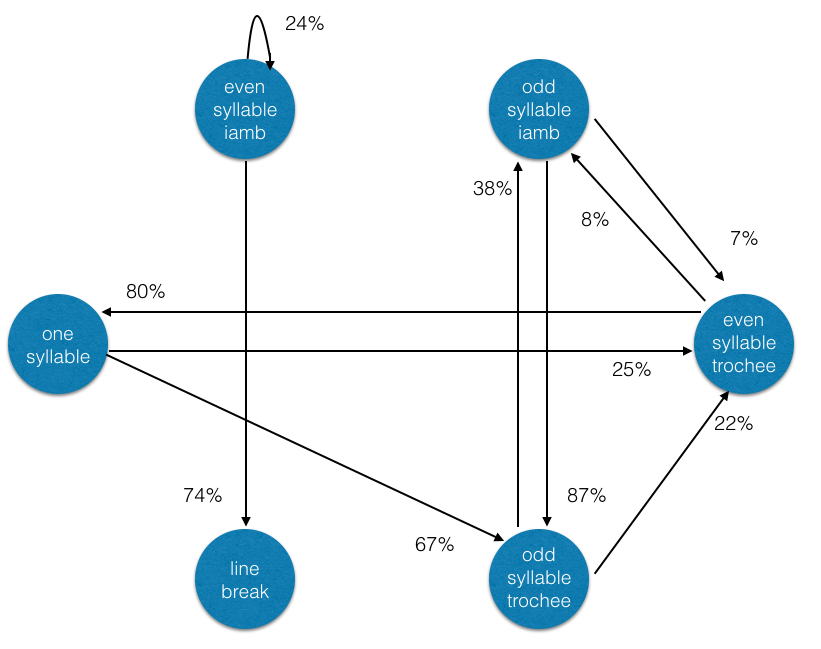
\includegraphics[scale=0.5]{transitions.png}

    One syllable words are not that interesting because they can be either stressed
    or unstressed in the meter. For even syllable iambs we see that they almost always
    transition to another even syllable iamb or a line break, which fits in with
    iambic meter. Odd syllable iambs most commonly transition to trochees, which
    again makes sense. Even syllable trochees tend to transition to one syllable 
    words, which is fine since one syllable words can be stressed or unstressed.
    Odd syllable trochees most commonly transition to iambs, which fits the meter,
    but they also transition a fair amount to trochees, which isn't incorrect
    (the model is certainly not perfect). Other than that one outlying case though,
    there is clearly strong evidence that the HMM is capable of learning the
    meter present in the sonnets. \\

    We also listed the 20 most common words for each of these states. As you can see despite these states being highly correlated with certain metrical feet, they still are most likely to generate common words. This is likely due to
    the fact that there is less variety in the English language among articles
    and prepositions, which tend to have one syllable, than among nouns and
    verbs, which are more likely to have multiple syllables (and thus be able
    to be classified as an iamb or trochee). In summary, the trends described
    above will be difficult to identify by looking at the top 20 most likely words
    for each state because of how the input data is distributed.

\begin{tabular}{|c|c|c|c|c|c|}
    \hline
    One Syllable & Even Iamb & Odd Iamb & Odd Trochee & Even Trochee \\
    \hline
    so & that & NEWLINE & be & my \\
    to & the & part & thee & the \\
    i & in & eyes & me & thy \\
    or & then & not & love & in \\
    as & all & seen & will & to \\
    who & for & spent & away & do \\
    for & yet & place & sight & so \\
    why & by & doth & night & his \\
    they & which & did & mind & your \\
    making & having & may & pride & it \\
    with & if & woe & face & is \\
    the & look & like & make & every \\
    it & how & sight & see & can \\
    how & so & away & heart & not \\
    what & you & desire & NEWLINE & most \\
    since & she & stay & fair & doth \\
    nor & when & new & end & sweet \\
    sweet & sweet & still & days & that \\
    mad & nothing & friend & dead & by \\
    then & what & up & find & will \\
    \hline
\end{tabular}


\end{itemize}


\section{Additional Goals}
\medskip
\begin{itemize}


    \item \boldline{Rhyme} \\

        We wrote a special function to determine if two words rhymed or did not rhyme. To do this, we used the CMU rhyming dictionary utility to break words down into individual phonemes. We then checked to make sure the last vowel sound in both words was the same, and that all consonant sounds that came after that sound were identical. If a pair of words passed this test (for any combination of pronunciations listed by the CMU dictionary) we specified that they rhymed. After using this rhyming helper to generate sonnets, we noticed some multi-syllable words with a shared suffix, such as 'breaking' and 'buying', would register as a rhyme, even though they didn't sound right together. We added the additional constraint that the last two vowel sounds of multi-syllable words must be the same for them to rhyme. (We put this function in our file wordtools.py)

    \item \boldline{Meter (Counting syllables)} \\

        We also wrote a special tool (also in wordtools.py) to determine the number of syllables in a word. This was important for the line generator to be able to produce lines which had a fixed number of syllables. We initially counted the vowel sounds in the CMU dictionary pronunciation of a word to serve as the number of syllables, but we noticed that some of the more antiquated words used by Shakespeare were not present in the CMU dictionary. To work around this, we implemented an edge case where we counted vowel clusters in a word to determine the number of syllables.



\end{itemize}



\section{Conclusion}
\medskip
\begin{itemize}

    \item \boldline{Observations} \\

    Multiple times throughout this process we encountered a decision point 
    where we could remain faithful to generating organic lines from the HMM
    model or `cheat' by forcing the HMM to do a certain thing that we wanted it
    to do. Throughout this project we tried to err on the side of letting the 
    HMM do things by itself in order to increase the variety and authenticity
    of the lines we generated, instead of writing something that simply copied
    Shakespeare with minor variations and rearrangements. \\

    For example, in our initial implementation we achieved 10-syllable lines
    by counting the number of syllables after each emission and halting when
    the number of syllables equalled 10. If we exceeded 10, we would remove
    the last word and keep generating words until we hit 10 syllables exactly.
    This was bad not only because it biased the lines towards ones ending in
    one or two syllable words, but also because we were artificially ending
    the line instead of allowing the HMM to observe a transition to a line break
    and generate that transition organically. We were able to achieve these by
    adding line break tokens to our input sequences, and generating lines by
    iterating until the HMM output a line break token. We noticed a markable
    increase in the quality of our lines after this change, with far more
    nouns at the end of lines instead of conjunctions or articles.


    \item \boldline{Challenges} \\
    
    One of the biggest weaknesses with our current model design is that we 
    don't have any sort of continuity between lines. Because of how we broke
    the sonnets into sequences at the line level, each sequence ends with a 
    line break token, so there is no way to pass the state of the previous
    line on to the next line. This design choice was made in order to model
    the end of lines more accurately, as described above. But is has the trade
    off of disrupting the continuity of the poem. We couldn't come up with a
    design solution that allowed us to enjoy both of these benefits simultaneously,
    but it was definitely the biggest compromise we had to make throughout the 
    process. If we continued to work on the project this would be one of the
    first things that we would fix. 

    \item \boldline{Concluding Remarks} \\
    
    Our model is able to generate 14-line sonnets with 10-syllable lines that
    follow the ABABCDCDEFEFGG rhyme scheme of a sonnet. Each line is generated
    organically by an HMM, using no manipulation to get it into the correct
    form. Individual lines are pieced together to fit the rhyme scheme and
    poem length, but each rhyming word was generated organically by the HMM
    with no seeding involved. Meter and part-of-speech transitioning were
    both left to the HMM to model, and as demonstrated in the visualization 
    section the model is clearly attempting to represent these sonnet
    characteristics accurately. On the whole, we were very satisfied with 
    how this project went.
\end{itemize}

Poem Progression:

%TODO ADD POEMS
\end{document}
